\indent

Markov Chain Monte Carlo (MCMC) is a Monte Carlo sampling technique for generating samples from an arbitrary distribution.

The samples are not independent, but from a Markov chain where the future depends on upon the present.

Two popular implementations of MCMC are:

\begin{itemize}
    \item Metropolis-Hastings algorithm and generalization by Hastings
    \item Gibbs samplers
\end{itemize}

\subsection{Markov Chain}

\indent 

Markov chain is a random (stochastic) process that follows the Markov property. Markov property means that the future state of the process only depends on the current state. Consider a sequence $\{X_1,\ldots,X_n\}$, probabilities $P(X_n|X_{n-1},\ldots,X_1) = P(X_n|X_{n-1})$.

Three key components:
\begin{itemize}
    \item \textbf{State space}: Set of all possible states
    \item \textbf{Transition matrix}: Probabilities of moving from one state to another
    \item \textbf{Random sequence}: A sequence of random variables $(X_0,X_1,\ldots,)$
\end{itemize}

\subsubsection{Modelling Future Weather Conditions}

\indent 

\begin{figure}[h!]
    \centering
    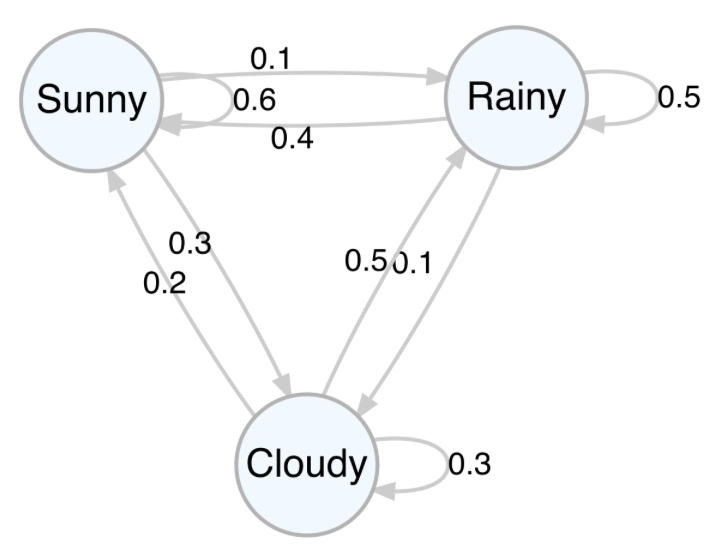
\includegraphics[width=0.5\linewidth]{Figure/Week 11/Modelling Future Weather Conditions.png}
    \caption{Modelling Future Weather Conditions}
\end{figure}

The state space is $S=\{\text{Sunny,Cloudy,Rainy}\}$, represented as the vertices of the graph. Edges represent the probability of moving from one state to another state. Example: if it is sunny today, 10\% chance of being rainy tomorrow.

The transition matrix $P$ is a $3\times 3$ matrix. Rows represent current state
Columns represent next state. $P_{ij}$ : probability of transiting from state $i$ to state $j$. Row of $P$ $\sum P_{i} = 1$.

\begin{align*}
    P = 
    \begin{pmatrix}
        0.6 & 0.1 & 0.3\\
        0.4 & 0.5 & 0.1\\
        0.2 & 0.5 & 0.3
    \end{pmatrix}
\end{align*}

This sequence is called a Markov Chain because each day’s weather only depends on today’s weather, not the entire history.

\subsubsection{Invariant (Stationary) Distribution}

\indent 

An invariant distribution is a probability distribution $\pi$ such that: $\pi = \pi P$ and $\pi \mathbf{1} = 1$.

If the system starts in distribution $\pi$, it stays in distribution $\pi$ after any number of transitions. It represents the long-term behavior of the Markov Chain. This is satisfied if the Markov chain is: Irreducible or Aperiodic.

\subsubsection{Irreducible}

\indent 

A Markov chain or transition matrix $P$ is said to be irreducible if there is some way of getting from state $i$ to state $j$, AND there is some way of getting from state $j$ to state $i$, $\forall i,j\in S$.

Consider the following transition matrix:

\begin{align*}
    P = 
    \begin{pmatrix}
        0 & 1 & 0\\
        0 & 0 & 1\\
        1 & 0 & 0
    \end{pmatrix}
\end{align*}

The chain cycles through: $1\rightarrow 2\rightarrow 3\rightarrow1\rightarrow 2\rightarrow 3\rightarrow\ldots$. You can return to the starting state only after $3, 6, 9, \ldots$ steps. Thus, \textbf{greatest common divisor} $\textbf{(gcd)}(3,6,9,...)=3$. All states are periodic with period 3.

\subsubsection{Aperiodic}

\indent 

Suppose we modify the transition matrix:

\begin{align*}
    P = 
    \begin{pmatrix}
        0.1 & 0.9 & 0\\
        0 & 0.5 & 0.5\\
        0.4 & 0 & 0.6
    \end{pmatrix}
\end{align*}

The state is aperiodic, meaning returns can happen more irregularly without being locked into a repeating cycle. Now can return in $1, 2, 3, 4, \ldots$ steps. $\textbf{gcd}(1,2,3,4,\ldots)=1$.

\subsubsection{The Use of Invariant Markov Chain}

\indent 

Similar to Monte Carlo, our main interest here continues to be the simulation of $X_1,X_2,\ldots$, that follow (or approximately follow) the distribution with density $f(x)$ where directly simulating from $f(x)$ is difficult.

This problem is ubiquitous in Bayesian statistics.

\begin{itemize}
    \item Frequentist statistics: there exist true parameters ($\boldsymbol{\theta}$ is fixed but unknown).
    \item Bayesian statistics: all model parameters are random variables.
\end{itemize}

For Bayesian statistics, the model parameters $\boldsymbol{\theta}$ has a prior distribution.

Given data $\mathbb{D}$, we want to compute the posterior distribution $p(\boldsymbol{\theta}|\mathbb{D})$.

\begin{align*}
    p(\boldsymbol{\theta}|\mathbb{D}) = \frac{p(\mathbb{D}|\boldsymbol{\theta})p(\boldsymbol{\theta})}{\int p(\mathbb{D}|\boldsymbol{\theta'})p(\boldsymbol{\theta'})d\boldsymbol{\theta'}}
\end{align*}

Generally, it’s very difficult to exactly compute $p(\boldsymbol{\theta}|\mathbb{D})$. Sample from $p(\boldsymbol{\theta}|\mathbb{D})$: using MCMC

Idea: construct a Markov chain such that its stationary distribution is the desired posterior distribution $p(\boldsymbol{\theta}|\mathbb{D})$.

\subsection{MCMC - Metropolis-Hasting algorithm}

\indent 

Imagine you are a politician trying to visit all the town halls in your electorate. Imagine there are four town halls: A, B, C, and D. Each town hall has a different number of voters. Your goal: Spend time at each town hall proportional to its voter population.

\begin{table}[h!]
    \centering
    \begin{tabular}{ccc}
        \hline
        \textbf{Town Hall} & \textbf{Number of Voters} & \textbf{Proportion (Target $f(x)$}\\\hline
        A & 500 & 0.25\\
        B & 1000 & 0.5\\
        C & 300 & 0.15\\
        D & 200 & 0.10\\\hline
    \end{tabular}
\end{table}

\step Start at a random town hall.

\step Propose moving to a randomly chosen new town hall.

\step Accept or reject the move:
\begin{itemize}
    \item If the new hall has more voters $\rightarrow$ Always accept.
    \item If fewer voters $\rightarrow$ Accept with probability
\end{itemize}

\begin{align*}
    \text{Accept probability} = \min \left(1,\frac{\text{Number of people in new town hall}}{\text{Number of people in current town hall}}\right)
\end{align*}

\step Repeat the process for a large number of steps (e.g., 10000).

\step Track the proportion of time spent in each town hall.

\subsubsection{Explanation}

\indent 

Similar to the acceptance-rejection method. It simulates a trial state. Accepts or rejects the trial state according to some random mechanism

Uses the Markov chain because each trial state depends on the previous state – Almost memory-less system. Aim is to construct a Markov chain $\{X_t,t=0,1,\ldots\}$ such that the limiting distribution is $f(x)$.

\subsubsection{Generalisation}

\indent 

We want to simulate samples from a complicated target distribution $f(x)$, which might be difficult to sample from directly.

\noindent \textbf{Basic Steps}:

\step Start with an initial state $X_0$.

\step Propose a new point $Y$ based on the current point $X_t$, using a proposal distribution $q(y|x)$.

\step Accept or reject the proposal $Y$ according to an acceptance probability $\alpha(X_t,Y)$.

This way, even if $q$ isn’t perfect, we still eventually generate samples that have the correct distribution $f(x)$ when it reaches stationarity.

\begin{algorithm}[H]
\caption{Metropolis-Hastings algorithm}
\begin{algorithmic}
    \For{$t=0,1,\ldots, N-1$}
        \State Draw $Y\sim q(x|X_t)$.
        \State Calculate acceptance probability $\alpha(X_t,Y)$.
        \State Define $\alpha(x,y) = \min\{\frac{f(y)q(x|y)}{f(x)q(y|x)},1\}$.
        \State Draw $U\sim \text{Uniform} (0,1)$.
        \State If $U\leq \alpha$ then $X_{t+1} \leftarrow Y$ else $X_{t+1}\leftarrow X_t$
    \EndFor
    \Ensure $X_1,X_2,\ldots,X_N$
\end{algorithmic}
\end{algorithm}

\subsubsection{Symmetric Proposal Function}

\indent 

If the proposal density function is $\textbf{symmetric}\Rightarrow q(y|x) = q(x|y)$. The acceptance probability has a simpler form. The MCMC algorithm is also known as a random walk sampler.

One common choice of a symmetric proposal function is just the Gaussian function, i.e., $q(x)\sim \mathcal{N}(x_t,\sigma)$. The choice of $\sigma$ affects how quickly the state space is explored.

\subsection{Applications of MCMC}

\indent

One common application of MCMC is to draw from the posterior distribution in Bayesian statistical methods.

\begin{align*}
    \textcolor{red}{P(A|B)} = \textcolor{blue}{\frac{P(B|A)}{P(B)}}\textcolor{orange}{P(A)}
\end{align*}

\begin{itemize}
    \item Posterior $\textcolor{red}{P(A|B)}$: The likelihood of $A$ occurring given $B$ has occurred.
    \item Likelihood ratio $\textcolor{blue}{\frac{P(B|A)}{P(B)}}$: The support $B$ provides for $A$.
    \item Prior $\textcolor{orange}{P(A)}$: The probability of $A$ before any data are gathered.
\end{itemize}

\subsubsection{The posterior distribution}

\indent 

Can use the Bayes rule for modelling and data.

\begin{align*}
    \textcolor{red}{P(\boldsymbol{\theta}|\mathbb{D})} = \textcolor{blue}{\frac{P(\mathbb{D}|\boldsymbol{\theta})}{P(\mathbb{D})}}\textcolor{orange}{P(\boldsymbol{\theta})}
\end{align*}

\begin{itemize}
    \item Posterior $\textcolor{red}{P(\boldsymbol{\theta}|\mathbb{D})}$: The likelihood of $\boldsymbol{\theta}$ occurring given the data $\mathbb{D}$.
    \item Likelihood ratio $\textcolor{blue}{\frac{P(\mathbb{D}|\boldsymbol{\theta})}{P(\mathbb{D})}}$: The support $\mathbb{D}$ provides for $\boldsymbol{\theta}$.
    \item Prior $\textcolor{orange}{P(\boldsymbol{\theta})}$: The probability of $\boldsymbol{\theta}$ before any data are gathered.
\end{itemize}

Typically $p(\mathbb{D})$ is a difficult integral to evaluate:

\[
p(\mathbb{D}) = \int P(\mathbb{D}|\boldsymbol{\theta}) p(\boldsymbol{\theta})d\boldsymbol{\theta}
\]

\subsubsection{MCMC for Estimating Regression Models}

\indent 

\begin{align*}
    \textcolor{red}{P(\boldsymbol{\theta}|\mathbb{D})} = \textcolor{blue}{\frac{P(\mathbb{D}|\boldsymbol{\theta})}{P(\mathbb{D})}}\textcolor{orange}{P(\boldsymbol{\theta})}
\end{align*}

\begin{align*}
    & Y = \beta_0+\beta_1X_1+\ldots+\beta_pX_p+\epsilon; & \epsilon\sim \mathcal{N}(0,\sigma^2)
\end{align*}

\begin{itemize}
    \item $\boldsymbol{\theta} = \{\beta_0,\beta_1,\ldots,\beta_p,\sigma^2\}$
    \item $\mathbb{D} = \{Y_1,Y_2,\ldots,Y_n,X_{11},X_{12},\ldots,X_{np}\}$
    \item $p(\mathbb{D}|\boldsymbol{\theta})$ will be Gaussian
    \item $p(\mathbb{D})$ is not so easy to compute
    \item $p(\boldsymbol{\theta})$ is the chosen prior
\end{itemize}

Recall the acceptance probability in the Metroplos-Hasting algorithm is:

\[
\alpha(x,y) = \min\left\{\frac{f(y)q(x|y)}{f(x)q(y|x)},1\right\}
\]

Assume the proposal density is symmetric, i.e.,  $q(y|x) = q(x|y)$. My target density $f$ is now the posterior distribution, i.e., $p(\boldsymbol{\theta}|\mathbb{D})$. Then in the Metropolis-Hastings algorithm, we only need to calculate:

\[
\alpha = \frac{p(\boldsymbol{\theta'|\mathbb{D}})}{p(\boldsymbol{\theta}|\mathbb{D})}=\frac{p(\mathbb{D}|\boldsymbol{\theta')}p(\boldsymbol{\theta'})}{p(\mathbb{D}|\boldsymbol{\theta})p(\boldsymbol{\theta})}
\]

Since $p(\mathbb{D)}$ doesn’t depend on $\boldsymbol{\theta}$, it cancels out on the right hand side of the above formula and hence it isn’t included in the formula.

\subsubsection{MCMC for Estimating $P(\text{Head})$ of a coin flip}

\indent 

Observe a series of coin flips: H, T, H, H, T, H, T, H, H, T, H, H, H, T, H, H, H, T, H, H, $\ldots$. $\theta = P(\text{Head})$

Frequentist perspective: $\theta$ is fixed but unknown.

Bayesian perspective: $\theta$ is a random variable; one can compute the likelihood of $\theta$ given the observed data.

$\theta_0$ set as an initial point. Compute $\theta_t$ as a Markov chain. Use MCMC algorithm to estimate the posterior distribution of $\theta$.

\subsubsection{MCMC practical considerations}

\indent 

The samples at the start of the MCMC, before the algorithm converges to the true distribution are known as the burn-in period. It should be discarded.

The samples generated by MCMC are correlated since they are from a Markov chain
Previously, many practitioners advocated thinning the samples by taking say every $k^{th}$ sample. 

This was done for a few reasons historically. Reduce correlations and compute standard errors more easily. Less space needed to store the chain.
